\chapter[Machines d'états finis]{Automates\\ {\it Machines d'états finis}}
\minitoc
%====================================================
\section{Introduction}
Parmi les circuits séquentiels précédemment évoqués, les automates ont une place privilégiée. Ces automates, appelés également
{\it machines d'états finis} ou encore {\it FSM (finite state machines)} permettent d'élaborer des circuits très complexes, de manière
simple et systématique. Par ailleurs, les automates sont un objet d'étude à part entière pour les informaticiens théoriciens, qui les utilisent
comme support à la modélisation de systèmes, y compris lorsque du logiciel prédomine dans ces systèmes : fondamentalement, tout système informatique
peut être considéré comme un (très gros) automate. Cette base conceptuelle solide pour les Electroniciens et les Informaticiens l'est aussi -- sans surprise-- pour les Automaticiens.
Les automates sont essentiels aux
systèmes embarqués : ils assurent à la fois la notion de séquencement ainsi que les tâches de contrôle
de dispositifs. Dans un premier temps, nous reviendrons sur des rappels concernant ces automates.
Dans un second temps nous calculerons les équations logiques constitutives de ces FSM.

\section{Machines d'états finis}
Il y a lieu de distinguer deux types d'automates : Moore et Mealy. Très proches conceptuellement, il est toutefois nécessaire de
bien comprendre leurs différence pour l'Ingénieur Numéricien. Nous verrons notamment que le couplage de tels automates peut-être source
de tracasseries délicates.

\paragraph{Automate de Moore}

Une automate de Moore est un sextuplet $(Q, \Sigma, \Delta, \sigma, \lambda, q_0 )$ :
\begin{itemize}
\item $Q$ est un ensemble fini d’états, $q_0$ est l’état initial
\item $\Sigma$ est l’alphabet d’entrée, $\Delta$ est l’alphabet de sortie
\item $\delta$ est une application de $Q \times \Sigma $ dans $Q$
\item $\lambda$  est une application de $Q$ dans $\Delta$, donnant la sortie associée à chaque état
\end{itemize}

La sortie de l'automate de Moore en réponse à une entrée $a_1 a_2\dots a_n$ , $n \geq 0$ est
$\lambda(q_0),\lambda(q_1)\dots \lambda(q_n)$ où
$q_0 ,\dots, q_n$ est la séquence d’états tels que $\lambda(q_{i-1},a_i) = q_i$ pour $1 \leq i \leq n$.
Remarque: Un automate de Moore retourne la sortie $\lambda(q_0)$ pour toute entrée.

\paragraph{Automate de Mealy}

Une automate de Mealy est un sextuplet $(Q, \Sigma, \Delta, \sigma, \lambda, q_0 )$ :
\begin{itemize}
\item $Q$ est un ensemble fini d’états, $q_0$ est l’état initial
\item $\Sigma$ est l’alphabet d’entrée, $\Delta$ est l’alphabet de sortie
\item $\delta$ est une application de $Q \times \Sigma $ dans $Q$
\item $\lambda$  est une application de $Q\times \Sigma$ dans $\Delta$, donnant la sortie associée à chaque état
\end{itemize}

$\lambda(q, a)$ donne la sortie associée à une transition d’un état q sur l’entrée a.
La sortie de l'automate de Mealy,en réponse à une séquence d’entrées $a_1,\dots a_n$ est
$\lambda(q_0, a_1) \lambda(q_1 , a_2 ) \dots \lambda(q_{n-1}, a_n)$
où $q_0 , q_1 ,\dots, q_n$ est la séquence des états tels que
$\lambda(q_{i-1}, a_i) = q_i$ pour $1 \leq i \leq n$.

\begin{figure}[h!]
  \centering
  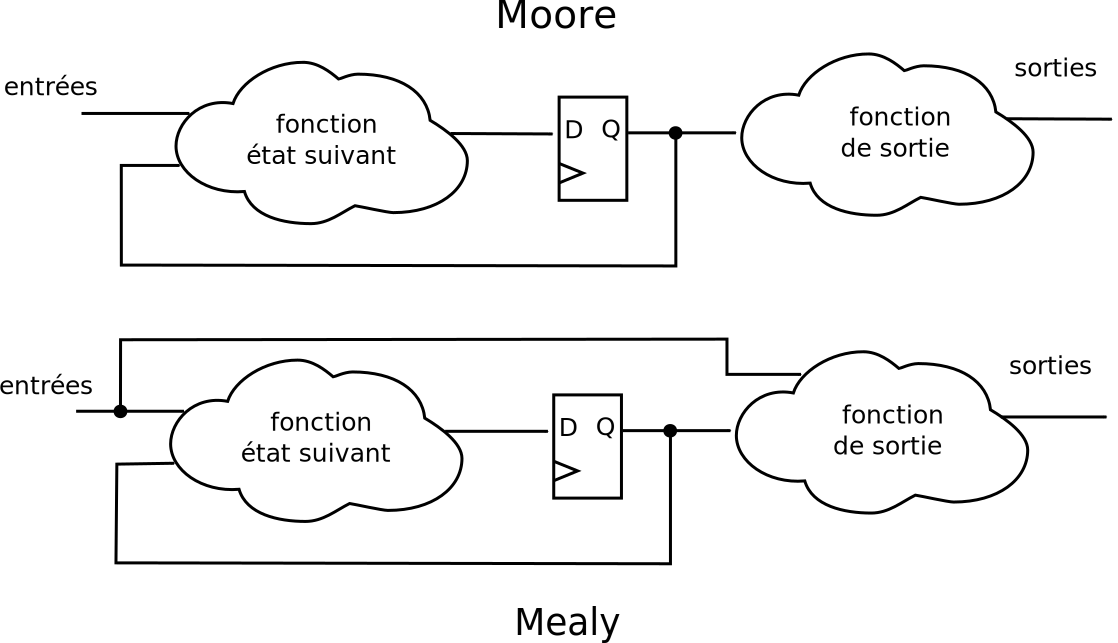
\includegraphics[scale=0.25]{./figures/moore_mealy.png}
  \caption{Automates de Moore et de Mealy}
  \label{fig:mealy_moore}
\end{figure}

\paragraph{Comparaison}
Les deux définitions sont très proches l'une de l'autre. On doit seulement comprendre que dans le cas d'une machine de Mealy, les sorties
dépendent des entrées et de l'état courant, alors que dans le cas de la machine de Moore, ces sorties dépendent uniquement de l'état courant.
En règle générale, les machines de Mealy sont plus rapides : leur chemin critique est plus court. Par contre, elles sont souvent proscrites des
bonnes règles de conception --en vigueur dans la plupart des sociétés-- car elles peuvent induire des bugs difficiles à localiser. En effet,
l'interconnexion de plusieurs automates de Mealy peut présenter des cycles combinatoires. On rappelle que ces cycles (ou boucles) combinatoires
sont interdites en logique synchrone car elle ne permettent pas de déterminer la fréquence propre de l'horloge du circuit.\\

En règle générale, toutefois, on plus code naturellement avec des machines de Mealy. La seule chose à prendre en compte est de bien clore le chemin
des sorties combinatoires par un registre adéquat. Cela fait partie des bonnes règles applicables par ailleurs : les entrées et les sorties d'un circuit
un tant soit peu complexe doivent être "clockées", c'est-à-dire échantillonnées dans des registres.

% \begin{figure}[h]
%   \centering
%   \includegraphics[scale=0.4]{./figures/comb_loops_mealy.png}
%   \caption{Composition d'automates de Mealy et risque de cycles combinatoires}
%   \label{fig:mealy_loops}
% \end{figure}

\paragraph{Exemple}
Nous présentons sur la figure \ref{fig:fsm} un exemple de FSM décrite à l'aide de bascule (ici une seule) et de portes logiques.
Les deux fonctions clés y sont représentées à savoir : la fonction d'état suivant et la fonction de sortie.
Malheursement, imaginer, concevoir, analyser et réaliser des automates à ce {\it niveau de détail} est sujet à erreur.
Par la suite, nous allons plutôt passer, {\it au préalable}, par une représentation plus adéquate, sur laquelle nous allons nous appuyer pour
établir les équations. Cette représentation est graphique ; nous l'appelerons "diagramme à bulles" ou diagramme états-transitions.
Elle est expliquée dans le paragraphe suivant. En TD, nous recoderons l'exemple \ref{fig:fsm} en diagramme états-transitions.
\begin{figure}[h]
  \centering
  \includegraphics[scale=0.4]{./figures/fsm-ex1.png}
  \caption{Exemple d'un automate matériel, réalisé à l'aide de portes logiques et (ici) d'une bascule D. En TD, nous tenterons de répondre à la question suivante : quel est le diagramme états-transitions équivalent ?}
  \label{fig:fsm}
\end{figure}

\section{Diagramme états-transitions}
Dans cette représentation graphique, un état est dénoté par un cercle, alors que les transitions sont représentées par
des flêches qui joignent les cercles. Il y a donc un état source et un état transition. Les transitions sont annotées par une expression booléenne qui indique la condition de changement d'état. Concernant les états, on indique
généralement le nom de l'état à l'intérieur du cercle (ou toute indications permettant de distinguer les états entre eux). Il existe également un état de démarrage, dénoté par un double cercle (ou parfois cible d'une flèche sans source).
L'automate évolue d'un état à l'autre, mais peut également réaliser des actions qui peuvent avoir lieu sur les transitions (Mealy) ou directement dans les états (Moore). Ces actions sont marquées ici après la double barre oblique.

\paragraph{Exemple : vending machine}
La figure \ref{fig:vending_machine} présente un automate appelé "vending machine". C'est un automate qui gère la délivrance d'un produit (soda, etc). Il se présente sous la forme d'un diagramme
états-transitions à 5 états. L'environnement immédiat de cet automate est un ensemble de capteurs et d'actionneurs. Ces derniers peuvent également se présenter sous la forme d'automates, de telle
sorte que c'est un ensemble complexe d'automates communicants qui constitue le système numérique complet. La FSM commande lé mécanisme de délivrance par deux signaux "open" et "close". Le mécanisme
de délivrance possède également un {\it timer} interne, non représenté ici qui décompte le temps à partir du moment où un ordre d'ouverture a été donné : lorsque le temps de délivrance (quelques secondes par exemple)
s'est écoulé, le signal "top" est à '1'. La FSM centrale est donc également sensible à cette entrée du mécanisme, de sorte que l'ensemble apparait comme bouclé.

\begin{figure}[h]
  \centering
  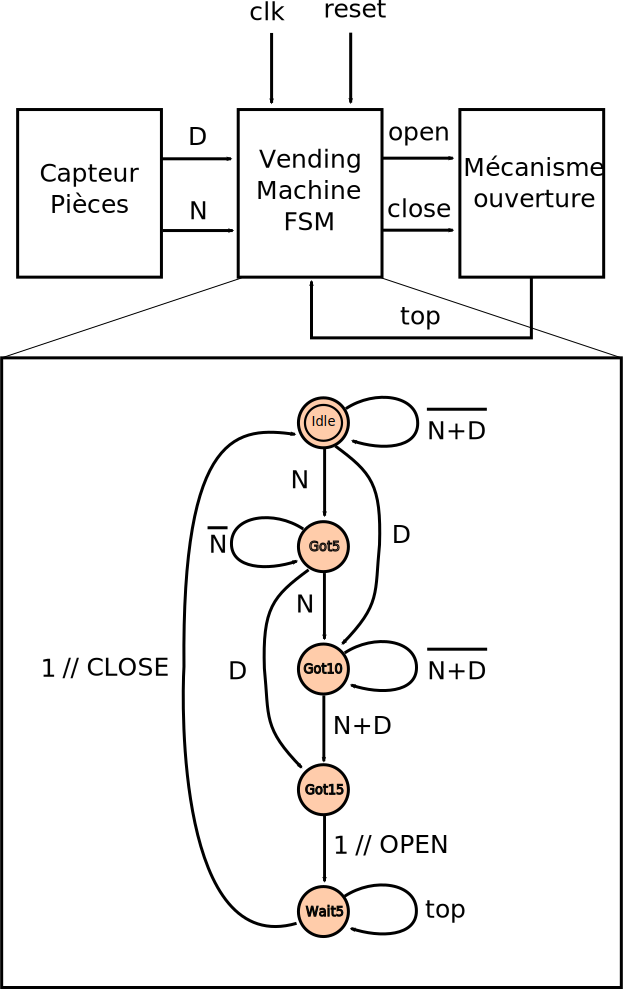
\includegraphics[scale=0.3]{./figures/vending_machine.png}
  \caption{Vending machine et son environnement}
  \label{fig:vending_machine}
\end{figure}

\section{Consistance ou {\it causalité} d'une machine d'états finis}

Pour que la FSM résultante soit considérée comme correcte ou ``consistante'', on doit examiner les
 transitions $c_i(s)$ partant de chaque état $s$ :
\begin{itemize}
\item \textbf{Réactivité} Les conditions sur les transitions doivent être {\it collectivement exhaustives} : il existe forcément une transition à '1'.
$$\forall s \in S : \sum_i c_i(s)=1$$
\item \textbf{Déterminisme} Les conditions sur les transitions doivent être {\it mutuellement exclusives} : on ne peut pas avoir deux transitions à '1' en même tem
ps.
$$\forall s \in S, \forall (i,j), i\neq j : c_i(s).c_j(s)=0$$
\end{itemize}

Cela signifie simplement que dans un état, il existe un, et un seul, état suivant.
Un tel automate, réactif et déterministe, est dit {\it causal}. Notons qu'un état peut avoir comme état suivant lui-
même : dans ce cas, le système décrit ne change pas d'état, tout simplement. \\

\section{Encodage des états}
Le diagramme états-transitions est une abstraction graphique qui est d'une grande aide lors de la conception amont.
Notamment, on a abstrait les états grâce à une simple bulle et un nom parlant ("symbolique"). Lors de la réalisation
concrète en Electronique, il faudra substituer cet état symbolique par un certain nombre de bascules qui "stockent" les bits d'états.
Il faut donc établir une correspondance (bijective) entre ces symboles et les codes binaires de ces états. Cette
correspondance s'appelle l'encodage des états. Là encore, il existe plusieurs manières de réaliser cet encodage.

\paragraph{Encodage dense}
L'encodage le plus naturel consiste à numéroter chacune des états en présence, pris dans un ordre arbitraire. La valeur binaire du numéro d'un état est
précisément le code de l'état. Cette manière de procéder conduit à une encodage dit "dense". Le terme "densité" utilisé
s'explique par le fait que le nombre de bascules résultant est restreint : pour $n$ états symboliques, on obtient
$\lceil \log_2(n) \rceil$ bascules. Observons le cas de la FSM "vending machine", et un encodage dense choisi. Pour 5 états
distincts, on a ici 3 bits d'états ; la densité est ici toute relative puisqu'avec 3 telles bascules, on pourrait encoder
jusqu'à 8 états.

\begin{table}[!htbp]
  \centering
  \begin{tabular}{|l|c|c|}
        \hline
        état  & numéro & code binaire  \\ \hline \hline
        Idle  & 0      & 000           \\ \hline
        Got5  & 1      & 001           \\ \hline
        Got10 & 2      & 010           \\ \hline
        Got15 & 3      & 011           \\ \hline
        Wait5 & 4      & 100           \\ \hline
    \end{tabular}
\end{table}

\paragraph{Encodage one-hot}
L'encodage {\it one-hot} ou, en français, "un bit par état", consiste à associer à chaque état d'une FSM de $n$ états
symbolique un code de $n$ bits de longueur. Cet encodage est de ce fait bien moins intuitif que l'encodage dense précédent.
Les bits d'un code "one-hot" sont particuliers : dans ce code, un seul bit est à '1' (tous les autres à '0'). Un exemple
d'un tel encodage est donné dans le tableau suivant.

\begin{table}[!htbp]
  \centering
  \begin{tabular}{|l|c|c|}
        \hline
        état  & numéro & code binaire  \\ \hline \hline
        Idle  & 1       & 00001           \\ \hline
        Got5  & 2       & 00010           \\ \hline
        Got10 & 4       & 00100           \\ \hline
        Got15 & 8       & 01000           \\ \hline
        Wait5 & 16      & 10000           \\ \hline
    \end{tabular}
\end{table}


\paragraph{Compromis temps-surface}

L'intérêt de l'encodage "one-hot" tient à la simplicité de conception des automates qui en découle.
Nous allons y revenir très bientôt. De plus les équations logiques des transitions, qui découleront, se révêlent plus simples (moins de portes logiques) et présentent
des chemins critiques plus courts que dans le cas de l'encodage dense.
Toutefois, étant donné le nombre plus important de bascules D engendrées dans le cas de l'encodage "one-hot",
il faudra calculer soigneusement les gains éventuels lors de l'attribution définitive de l'encodage.
En effet, on considère qu'une bascule D correspond à environ 10 portes logiques à 2 entrées (typiquement une porte AND). Ce nombre
peut notamment se révéler prohibitif en comparaison du nombre de portes engendrées dans le cas d'un encodage dense.
De même, signalons que ce seul encodage dense (et d'ailleurs tout encodage) est un choix, qui peut avoir des conséquences
insoupçonnées en ce qui concerne la simplification des équations qui en découleront. C'est un problème très complexe, qui a mobilisé
un grand nombre d'études théoriques jusque dans les années 1990.
Ce calcul est désormais automatisé dans les outils de synthèse, sous la forme d'heuristiques.

%====================================================
\section{Méthode générale de conception d'un automate}
On cherche à établir les équations logiques de l'automate : les équations logiques de la fonction état suivant,
ainsi que de la fonction de sortie. On doit établir une {\it table de vérité séquentielle} qui, à partir d'une présentation de l'ensemble des combinaisons de l'état courant et des entrées,
recense toutes les sorties, mais également l'état futur du système.On suggère ici de procéder en 2 étapes.

\paragraph{Table de vérité symbolique}
  La première consiste à conserver le nom {\it symbolique} des états tandis que la seconde fait a
pparaître l'{\it encodage} de ces états.

\begin{table}[!htb]
  \centering
  \begin{tabular}{|c|c|c|c||c|c|c|c|}
        \hline
        état courant & entrée 1 & ... & entrée n &  état suivant & sortie 1 & ... & sortie n \\ \hline
        IDLE        & ~    & ~     & ~            & ~            & ~        & ~   & ~    \\ \hline
        \dots       & ~    & ~     & ~            & ~            & ~        & ~   & ~    \\ \hline
        GOT5        & ~    & ~     & ~            & ~            & ~        & ~   & ~    \\ \hline
        \dots       & ~    & ~     & ~            & ~            & ~        & ~   & ~    \\ \hline
    \end{tabular}
\end{table}

%\FloatBarrier
\paragraph{Table de vérité explicite}

Cette énumération conduit donc à un nouveau tableau, encore plus explicite, où figurent, {\it à gauche}, les sorties $Q_i$ des bascules
--c'est l'état couran du système-- et, {\it à droite} les entrées $D_i$ de ces mêmes bascules. Pour établir cette
table de vérité séquentielle, on énumère toutes les valeurs possibles de la partie de gauche, et on calcule les sorties et les $D_i$.


\begin{table}[!htb]
  \centering
    \begin{tabular}{|c|c|c|c|c|c||c|c|c|c|c|c|}
        \hline
        $Q_n$ & \dots & $Q_0$ &  entrée 1 & ... & entrée n & $D_1$ & \dots & $D_0$ & sortie 1 & ... & sortie n \\ \hline
        ~   & ~    & ~  & ~  & ~  & ~  & ~  & ~  & ~        & ~   & ~ & ~        \\
        ~   & ~    & ~  & ~  & ~  & ~  & ~  & ~  & ~        & ~   & ~ & ~        \\
        \hline
    \end{tabular}
\end{table}

\section{Exemple complet}
Illustrons notre propos avec la FSM exposée sur la figure. Il s'agit d'un automate de de Moore car on constate que la sortie $f$ a lieu dans les états, et non sur les transitions.

\begin{figure}[h]
  \centering
  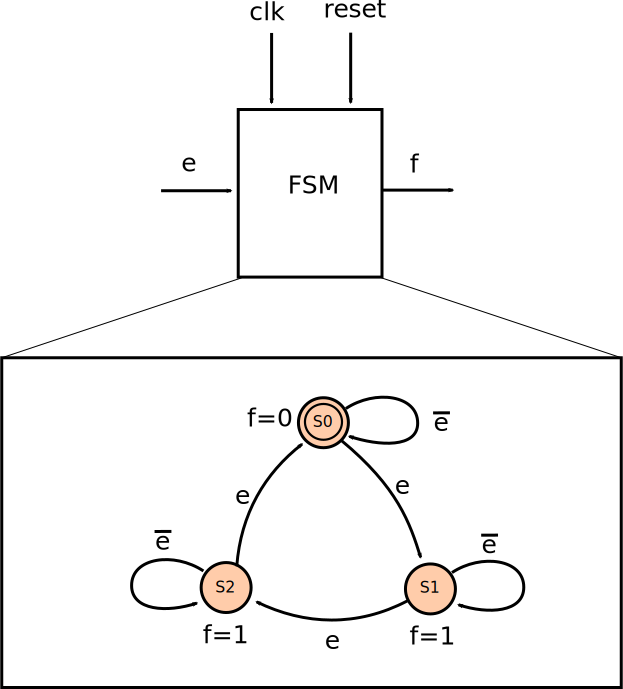
\includegraphics[scale=0.4]{./figures/exo_fsm.png}
  \caption{Tableaux de Karnaugh de l'exemple}
  \label{fig:karnaugh}
\end{figure}

\paragraph{Encodage}
La FSM présente 3 états. Choisissons un encodage dense :
\begin{table}[!htbp]
  \centering
  \begin{tabular}{|l|c|c|}
        \hline
        état  & numéro & code binaire  \\ \hline \hline
        S0  & 0       & 00           \\ \hline
        S1  & 1       & 01           \\ \hline
        S2  & 2       & 10           \\ \hline
    \end{tabular}
\end{table}

\paragraph{Table de vérité symbolique}
Passons à la table de vérité. On reporte les observations du schéma précédent.
\begin{table}[!htb]
  \centering
  \begin{tabular}{|c|c||c|c|}
        \hline
        état courant & e &  état suivant & f \\ \hline
        S0 & 0 & S0 & 0 \\ \hline
        S0 & 1 & S1 & 0 \\ \hline
        S1 & 0 & S1 & 1 \\ \hline
        S1 & 1 & S2 & 1 \\ \hline
        S2 & 0 & S2 & 1 \\ \hline
        S2 & 1 & S0 & 1 \\ \hline
    \end{tabular}
    \caption{Table de vérité avec nom explicite des états.}
    \label{fig:thruth_1}
\end{table}

\paragraph{Table de vérité avec encodage explicite}
Il en découle la table de vérité suivante.
\begin{table}[!htb]
  \centering
    \begin{tabular}{|c|c|c||c|c|c|}
        \hline
        $Q_1$ & $Q_0$ &  e & $D_1$ & $D_0$ & f \\ \hline
        0 & 0 & 0 & 0 & 0 & 0 \\ \hline
        0 & 0 & 1 & 0 & 1 & 0 \\ \hline
        0 & 1 & 0 & 0 & 1 & 1 \\ \hline
        0 & 1 & 1 & 1 & 0 & 1 \\ \hline
        1 & 0 & 0 & 1 & 0 & 1 \\ \hline
        1 & 0 & 1 & 0 & 0 & 1 \\ \hline
        1 & 1 & 0 & x & x & x \\ \hline
        1 & 1 & 1 & x & x & x \\ \hline
    \end{tabular}
    \caption{Table de vérité avec encodage explicite}
    \label{fig:thruth_1}
\end{table}

\paragraph{Tableaux de Karnaugh et Equations logiques}
On établit les 3 tableaux de Karnaugh, relatifs aux équations des 2 bascules et de la sortie. On effectue les regroupements simplificateurs, en profitant
des valeurs {\it don't care} 'X', que l'on peut positionner à '0' ou '1' de manière à créer des regroupements plus intéressants.
\begin{center}
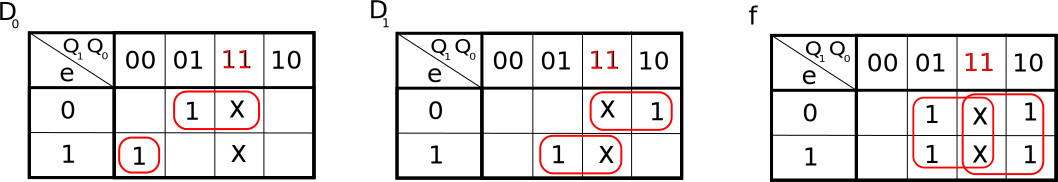
\includegraphics[scale=0.4]{./figures/exemple_table_k.png}
\end{center}

% \begin{figure}[h]
%   \centering
%   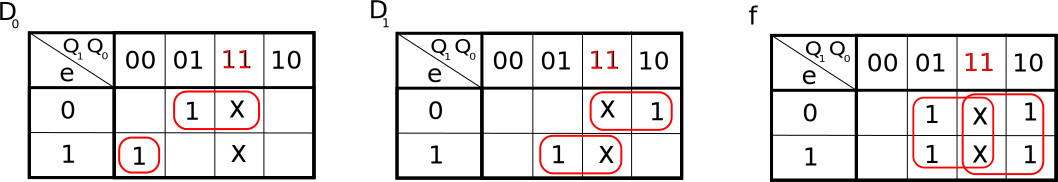
\includegraphics[scale=0.35]{./figures/exemple_table_k.png}
%   \caption{Tableaux de Karnaugh de l'exemple}
%   \label{fig:karnaugh}
% \end{figure}

Les équations obtenues, sont :
\begin{align}
 D_0 & = Q_0.\barre{e}+\barre{Q_1}.\barre{Q_0}.e \\
 D_1 & = Q_1.\barre{e}+Q_0.e \\
 f   & = Q_1 + Q_0 \\
\end{align}

\paragraph{Circuit électronique}
Le circuit réalisant l'automate exemple est donné sur la figure \ref{fig:circuit}. Notons qu'afin de ne pas surcharger le schéma, nous avons omis les fils
relatifs à l'initialisation des bascules D, ainsi que l'horloge.
\begin{figure}[h]
  \centering
  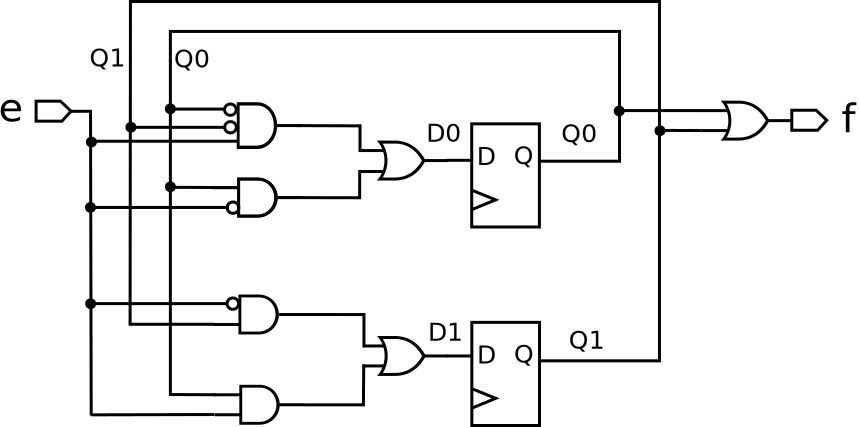
\includegraphics[scale=0.35]{./figures/fsm_circuit.png}
  \caption{Implémentation matérielle de l'automate}
  \label{fig:circuit}
\end{figure}


\section{Gérer la complexité }
\paragraph{Position du problème}

On se rend compte que le nombre d'entrées dans cette table de vérité grandit très vite : on se souvient alors que pour $n$ entrées, on devra avoir $2^n$ lignes d'énumérations
des combinaisons dans cette table. Cela ne devient plus gérable par un humain. Il faut automatiser.
Notons que le nombre précédent $2^n$ est indépendant du nombre des sorties ; la complexité des équations booléennes de ces sorties croît en fonction de $n$, ce qui n'est guère
rassurant : on pourra  avoir $2^n$ monômes dans ces équations. Bref : il faudra le plus souvent se résoudre à recourir à des synthétiseurs automatiques pour le calcul des équations ou recourir à des statégies plus intelligentes
que le calcul "brute force". Généralement, il est judicieux d'{\it observer} les relations qui existent entre les contraintes booléennes.

\paragraph{Contraintes mutuelles}

Ainsi, prenons le simple cas du dé électronique (dé à jouer, à 6 points maximum) : on verra en TD que ce dé peut être modélisé par une FSM. Pour simuler l'effet d'un dé qui est lancé, on appuie
sur un bouton. Pendant que le bouton est enfoncé, une FSM allume et éteint les diodes correspondant aux points du dé, en comptant de 1 à 6.
Avec une horloge dont la fréquence de fonctionnement est élevé, le joueur ne peut évidemment pas voir ce défilement. Lorsqu'il relâche le bouton, un chiffre est figé sur les points.
Logiquement, on s'attend à ce que l'on ait à établir 6 équations logiques : une équation par diode. On remarque toutefois que tous les points qui s'allument et s'éteignent
sur une face du dé sont interdépendants et des "symétries" apparaissent dans les équations. Ceci conduit à ne pas traiter 6 équations, mais
seulement quelques unes d'entre elles, les autres en découlant facilement. Nous garderons donc en mémoire qu'il faut un peu d'observation et de perspicacité pour traiter de tels
problèmes.

\section{Méthode particulière : cas de l'encodage {\it one-hot}}

\paragraph{Intuition} Il existe un cas particulier d'encodage qui permet d'éviter totalement la méthode générale précédente : l'encodage {\it one-hot}. Posons nous
la question de la signification de cet encodage : nous savons qu'il est appelé "un bit par état". Cela signifie qu'à un instant donné, une seule bascule
aura une sortie $Q_i$ à '1' ; nous connaissons donc instantanément, du fait de cette seule observation, dans quel état on se trouve.
Nullement besoin d'observer les autres valeurs (à '0') des autres bascules. On dit que la bascule en question est "allumée" lorsque sa sortie vaut '1' .
Si on observe désormais le fonctionnement de l'automate durant plusieurs coups d'horloges, on verra successivement s'allumer différentes bascules,
{\it l'une après l'autre} : tout se passe comme si un jeton se déplaçait d'une bascule à l'autre. Lorsque la bascule $i$ détient le jeton, l'automate se trouve dans l'état de numéro $i$ !



\paragraph{Obtention directe des équation} On peut utiliser les propriétés de cet encodage pour établir une correspondance {\it directe} entre le schéma initial et le circuit correspondant.
Dit autrement : il suffit d'observer le diagramme états-transitions de l'automate pour construire directement le circuit !
Pour cela, il suffit d'établir des règles simples :

\begin{itemize}
  \item On dessine une bascule $D$ pour un état $S$
  \item Pour chacune des transitions sortantes d'un état $S_i$ vers un état $S_j$, on dessine une porte AND connectée d'une part à la sortie $Q$ de la bascule de l'état $S_i$, et
  d'autre part la condition booléenne $c$ de la transition $S_i\rightarrow_{c} S_j$. Appelons $c_{i,j}$ la sortie de cette porte AND.
  \item Pour chacune des transitions entrantes d'un état $S_j$ on dessine une porte OR connectée à l'entrée $D_j$ et possédant autant d'entrées qu'il existe de transitions entrantes.
  A partir des états précedents $S_i$, on connecte le signal $c_{i,j}$ sur une des entrées de cette porte OR.
\end{itemize}

\begin{figure}[!htb]
  \centering
  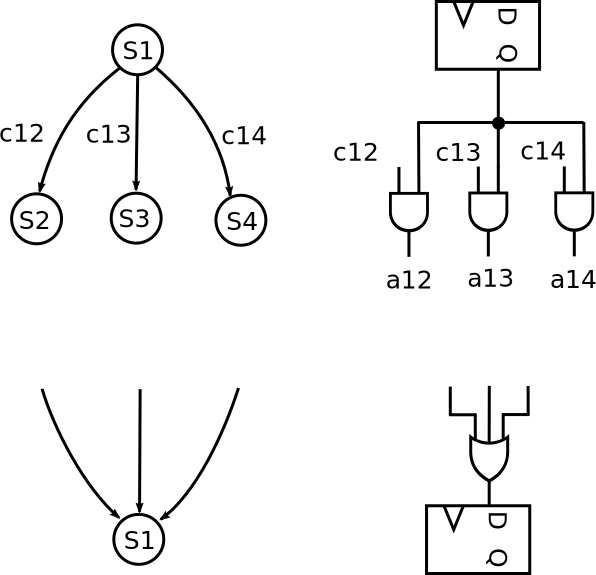
\includegraphics[scale=0.3]{./figures/one_hot_method.png}
  \caption{Procédé simplifiant la génération d'un circuit d'automate dans le cas d'un encodage {\it one-hot}.}
  \label{fig:one_hot}
\end{figure}

Ce schéma de traduction est très simple à mettre en oeuvre. Il est résumé sur la figure \ref{fig:one_hot} : on se borne à regarder le schéma et réécrire
les équations logiques des entrées $D_i$. Voici un exemple, sur la figure \ref{fig:one_hot2}.

\begin{figure}[!hbt]
  \centering
  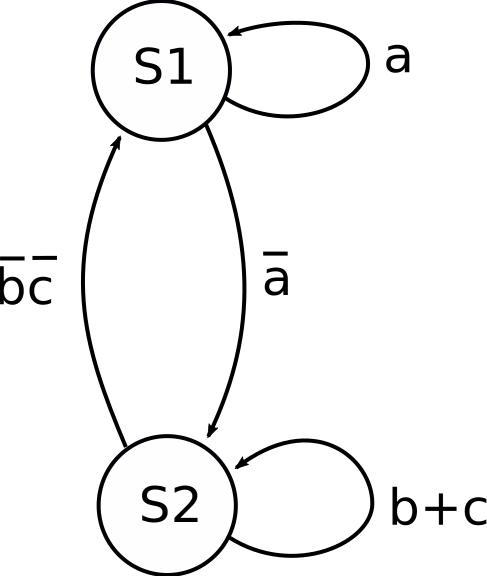
\includegraphics[scale=0.25]{./figures/fsm_one_hot.png}
  \caption{Exemple pour la méthode directe d'obtention des équations, à partir de l'encodage one-hot}
  \label{fig:one_hot2}
\end{figure}

Les équations sont directement obtenues :
$$
\begin{array}{lcl}
  D_1 & = & Q_1.a+Q_2.\overline{b}.\overline{c}\\
  D_2 & = & Q_2.(b+c)+Q_1.\overline{a}\\
\end{array}
$$

\section{A propos du caractère fondamental des automates}

Nous l'avons déjà mentionné : les automates sont des objets étudiés par différentes
communautés scientifiques. C'est un objet fondamental de l'Informatique, car il permet
de raisonner sur les évolutions temporelles d'un système : les automates sont à l'Informaticien (et l'Electronicien)
ce que les équations différentielles sont au Physicien. A titre d'illustration, observons le schéma de la figure \ref{sys1}. Cette figure décrit l'architecture d'un système-sur-puce (SoC : system-on-chip).
Un SoC est l'agglomération d'un ensemble de composants {\it sur un seule et même puce}. Généralement un processeur y tient un rôle central. Il est en communication
avec des périphériques de communication (clavier, écrans, ethernet), mais également des périphériques d'accélération de calculs le plus souvent dédiés. Cette
communcation s'effectue à travers un bus (et de plus en plus, à travers un NoC réseau-sur-puce). La complexité de l'ensemble est difficile à appréhender pour un humain.


\begin{center}
\begin{minipage}[t]{10cm}
 \centering
 \includegraphics[width=10cm]{./figures/system_1.png}
 \label{sys1}
\end{minipage}
\end{center}

\paragraph{} Toutefois, in fine, l'ensemble de ces éléments constitutifs ne représentent {\it que} des automates, comme l'illustre la figure suivante.
Ce socle est suffisamment solide pour que des outils dits de {\it verification formelle} permettent de vérifier les propriétés du système dans son ensemble.

\begin{center}
\begin{minipage}[t]{10cm}
 \centering
 \includegraphics[width=10cm]{./figures/system_2.png}
\end{minipage}
\end{center}

\section{Conclusion}
Ce chapitre nous a permis de découvir la notion d'automate matériel.
L'implémentation matérielle de tels automates peut être réalisée de manière quasi-mécanique, en mobilisant nos connaissances
en matière de logique combinatoire, tableaux de Karnaugh, mais également bascules D. Nous avons également abordé la notion de consistance
de ces automates : un calcul formel permet de s'assurer que notre automate a du sens. Ce calcul se fait au préalable de la réalisation
concrète du circuit. C'est là une propriété intéressante, liée à la logique booléenne, que l'on ne retrouve guère en matière logiciel. Là, le domaine
du matériel semble en avance sur le logiciel : notons toutefois qu'une classe de languages informatiques, dédiés à la réalisation de logiciels embarqués,
s'appuie sur les mêmes calculs et les mêmes raisonnements formels pour assurer la fiabilité des logiciels embarqués. Ces langages s'appellent {\it langages synchrones} : on comprend
désormais bien cette appellation ! Je vous invite notamment à lire, voir ou écouter les conférences de Gérard Berry, à l'Académie des Sciences.
Il illustre parfaitement, mieux que quiconque, ce propos.
